% !TEX root = tesis.tex

\chapter{Desarrollo de nueva electrónica para el SciCRT}
\chaptermark{Nueva electrónica}
\label{chap:tres}

Las necesidades del SciCRT operando en Sierra Negra no se acoplan directamente a los objetivos específicos de los experimentos K2K y SciBooNE, una de nuestras metas dentro de la colaboración ha sido el desarrollo de electrónica de alta velocidad de transferencia, bajo costo y consumo de potencia. Sumado a esto, hemos decido seguir principios similares a los del desarrollo de software libre para evitar el \emph{vendor lock-in}. No obstante, encontrar una solución que cumpla de forma simultánea todos estos requerimientos resulta muy complejo. En este capítulo abordaré detalladamente el desarrollo del sistema de adquisición de datos, dando particular énfasis a su motivación científica. En este sentido el primer punto a tratar será la velocidad de transferencia.

En \num{2015} desarrollamos nueva electrónica BE utilizando \emph{SiTCP} (procesador embebido programable desarrollado para experimentos de física de altas energías) y la instalamos en uno de los SB que componen las capas de neutrones del telescopio \cite{ysasai17}. Gracias al uso de esta tecnología logramos alcanzar una tasa de transferencia de datos \num{10} veces mayor a la que teníamos con el bus VME.

A continuación presento un estudio mediante simulación MC para evaluar el desempeño del SciCRT utilizando la electrónica de alta velocidad. Este análisis tiene también por objetivo mostrar la motivación detrás del requerimiento en la velocidad de transferencia. Hago notar que estudios similares se encuentran en: \cite{ynagai14,ysasai17}. El resultado original contenido en esta tesis lo presenté en la Conferencia internacional de Rayos Cósmicos en \emph{Busan}, Corea del Sur \cite{manzorena171}.

\section{Desempeño del SciCRT ante un evento de neutrones solares}

Evaluaremos la respuesta del SciCRT a un evento de neutrones solares mediante simulación MC, comparando el resultado con los datos obtenidos por TNS instalado en Sierra Negra durante la ráfaga del \num{7} de Septiembre de \num{2005} \cite{sako06}. Este evento fue detectado por el TNS con una significacia de $17\sigma$ en el canal de partículas neutras con energías mayores a $>\SI{30}{\mega\electronvolt}$. El pico de la emisión de rayos \emph{X} duros (satélite Integral) fue a las 17:36:40 UT. La figura

Si asumimos el flujo de neutrones solares para este evento, podemos estimar la significancia de las señales detectadas por el SciCRT en un evento similar. Para nuestra estimación consideraremos como parámetros de entrada \cite{ynagai14}: un espectro de energía de los neutrones en el Sol de acuerdo a una ley de potencias
$\num{6.1e27}\left(E/\si{\mega\electronvolt}\right)^{-3.8}\si{\per\mega\electronvolt\per\steradian}$, neutrones emitidos de manera impulsiva en el Sol y un ángulo cenital de \ang{17.5}. La propagación de los neutrones solares en la atmósfera terrestre se simula usando el modelo de Shibata.

\begin{figure}
\centering
  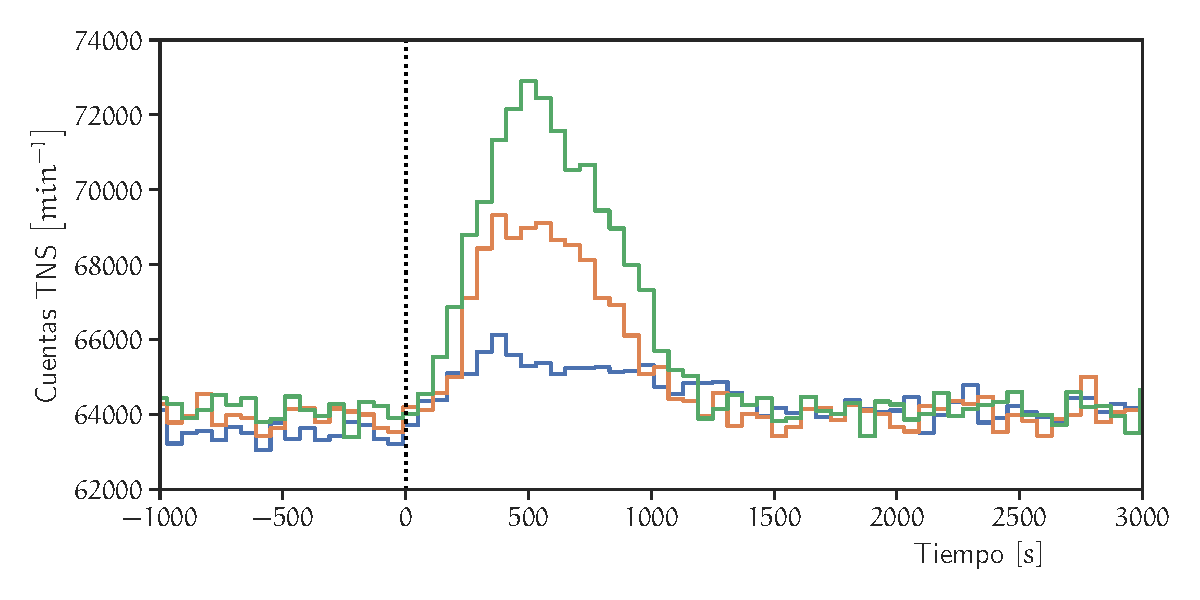
\includegraphics[width=\textwidth]{scicrt-sim.pdf}
  \caption{Simulación de los perfiles temporales del SciCRT asumiendo un flujo de neutrones solares similar al del evento del \num{7} de Septiembre de \num{2005}. La curva azul muestra los datos obtenidos por el TNS, la línea naranja es el perfil temporal del SciCRT usando la electrónica original. La línea roja muestra el caso cuando instalamos la electrónica de alta velocidad. Los datos están normalizados al nivel de fondo del TNS.}
  \label{fig:solar-sim}
\end{figure}

Los resultados de nuestro cálculo se muestran en la figura \ref{fig:solar-sim}. Es importante aclarar que para esta estimación tomamos en cuenta dos situaciones; una con la electrónica original y otra con la electrónica de alta velocidad, ambas instaladas en $4/8$ del detector. La línea punteada en \SI{0}{\second} indica el instante en que la intensidad de rayos \emph{X} duros alcanzó el máximo. En la figura la linea azul representa los datos del TNS de partículas neutras con $E_{k}>\SI{30}{\mega\electronvolt}$. El perfil temporal de las cuentas del SciCRT con la electrónica original (línea naranja) muestra una significacia de $39\sigma$, lo que se traduce en una sensibilidad $2.3$ veces mayor a la del TNS durante el mismo evento\footnote{La significacia del TNS para el evento fue estimada en $17\sigma$.}. Sin embargo, al tomar en cuenta el caso de la nuevo DAQ (línea verde), el incremento es de $59\sigma$, es decir, $3.5$ veces mayor sensibilidad.

Con respecto a los datos de energía depositada el incremento también notable puesto que se tiene una sensibilidad $3$ veces mayor, con la ventaja extra de que podemos estimar el espectro de los neutrones con una excelente resolución \cite{ysasai17}.

In the near future we plan to make further improvements on the detector, all of which will have a impact on the performance of the SciCRT. In the next brief list we summarize the currently undergoing tasks: $1\left.\right)$ implementation of a selective trigger mode which enables the suppression of pedestal data, $2\left.\right)$ further improvement of the throughput rate of the BEB, with the installation of more DAQ servers to control the data acquisition and $3\left.\right)$ development of new low-cost front-end electronics to enable the full installation of the SciCRT.

Despite this, the sensitivity to such transient events is function of the active volume and therefore of the total electronic units installed. Considering that only $3/8$ of the electronics are available at the present time, the development of new FEUs is a priority of our experiment to fully realize the capabilities of SciCRT as an improved SNT. Furthermore, given the operation of the telescope at high altitude, sustainable long term operation requires the production of low cost/low power electronics, since the severe environment condition reduce the useful life of the modules and hinder the disposal of waste heat.

\section{La técnica de \emph{Time over threshold}}

 Luego entonces la carga total depositada entonces se puede calcular como:

\begin{equation}
Q=\int_{0}^{\infty} i_{pmt}\left(t\right)\mathrm{d}t
\end{equation}

La corriente $i\left(t\right)$ se puede modelar como:

\begin{equation}
i\left(t\right)=i_{0} \exp\left(-\dfrac{t}{\tau_{d}}\right)
\end{equation}

donde $i_{0}$ es la corriente característica de la interacción y está definida como:

\begin{equation}
i_{0}=\lambda Q
\end{equation}

con $\lambda=\dfrac{1}{\tau_{d}}$. Finalmente, $i\left(t\right)$ se puede expresar de la siguiente manera:

\begin{equation}
i\left(t\right)=\lambda Q \exp\left(-\lambda t\right)
\end{equation}

El circuito que se requiere para realizar la integración del pulso y posteriormente registrar la altura de la señal integrada es complejo y no se adapta a las necesidades del SciCRT

Para simplificar la electrónica, buscamos desarrollar un sistema que utilice el Time over threshold. Primero debemos encontrar una relación entre la carga depositada y el tiempo que dura la señal encima de un umbral definido. Consideremos cuatro casos:

1. Sin utilizar circuito de formación
    1. Utilizando un umbral constante
    2. Utilizando un umbral variante en el tiempo
2. Utilizando circuito de formación
    1. Utilizando un umbral constante
    2. Utilizando un umbral variante en el tiempo

El problema de encontrar la relación entre $Q$ y $ToT$ se resuelve mediante un sistema de ecuaciones.

Consideramos $s\left(t\right)$ la señal del fotomultiplicador y $v\left(t\right)$ la función que describe al umbral.

\begin{figure}
        \centering
        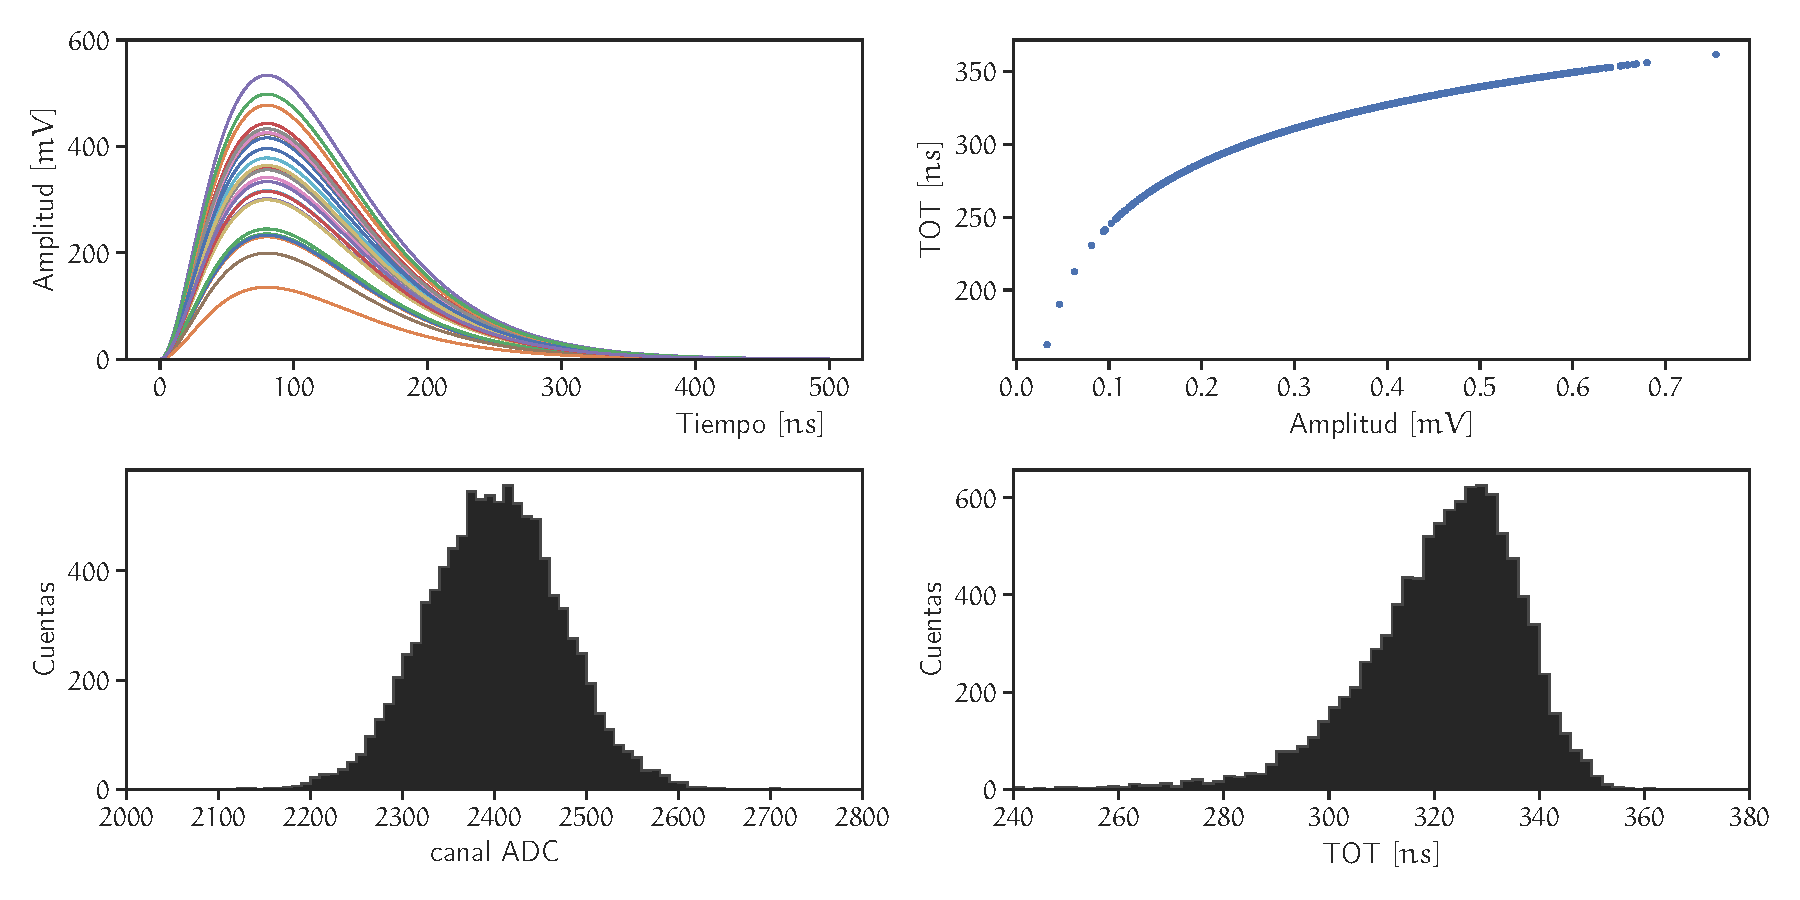
\includegraphics[width=\textwidth]{TOT-model.pdf}
        \caption{Modelo de primeros principios de conversión Carga-TOT.}
        \label{fig:tot-model}
\end{figure}

\begin{figure}
        \centering
        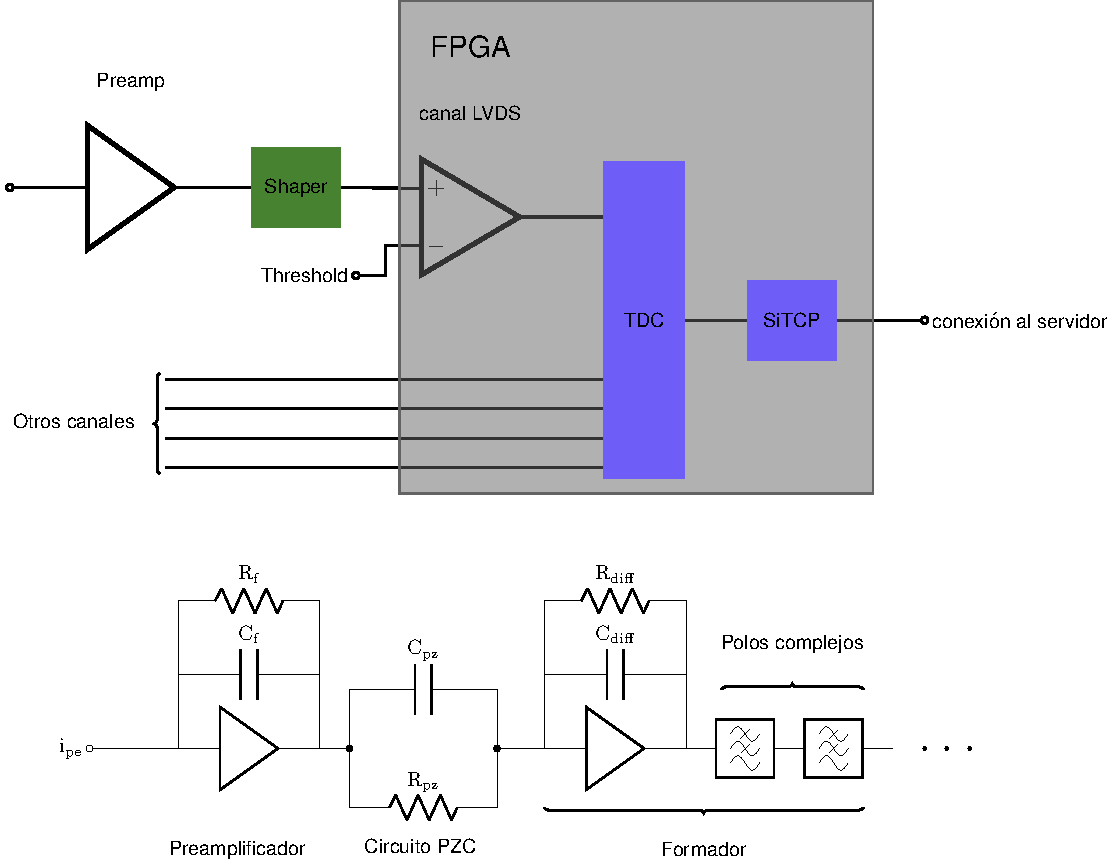
\includegraphics[width=\textwidth]{nfeb-prot.pdf}
        \caption{Diagrama esquemático de la nueva electrónica del SciCRT.}
        \label{fig:nfeb-prot}
\end{figure}


\begin{figure}
        \centering
        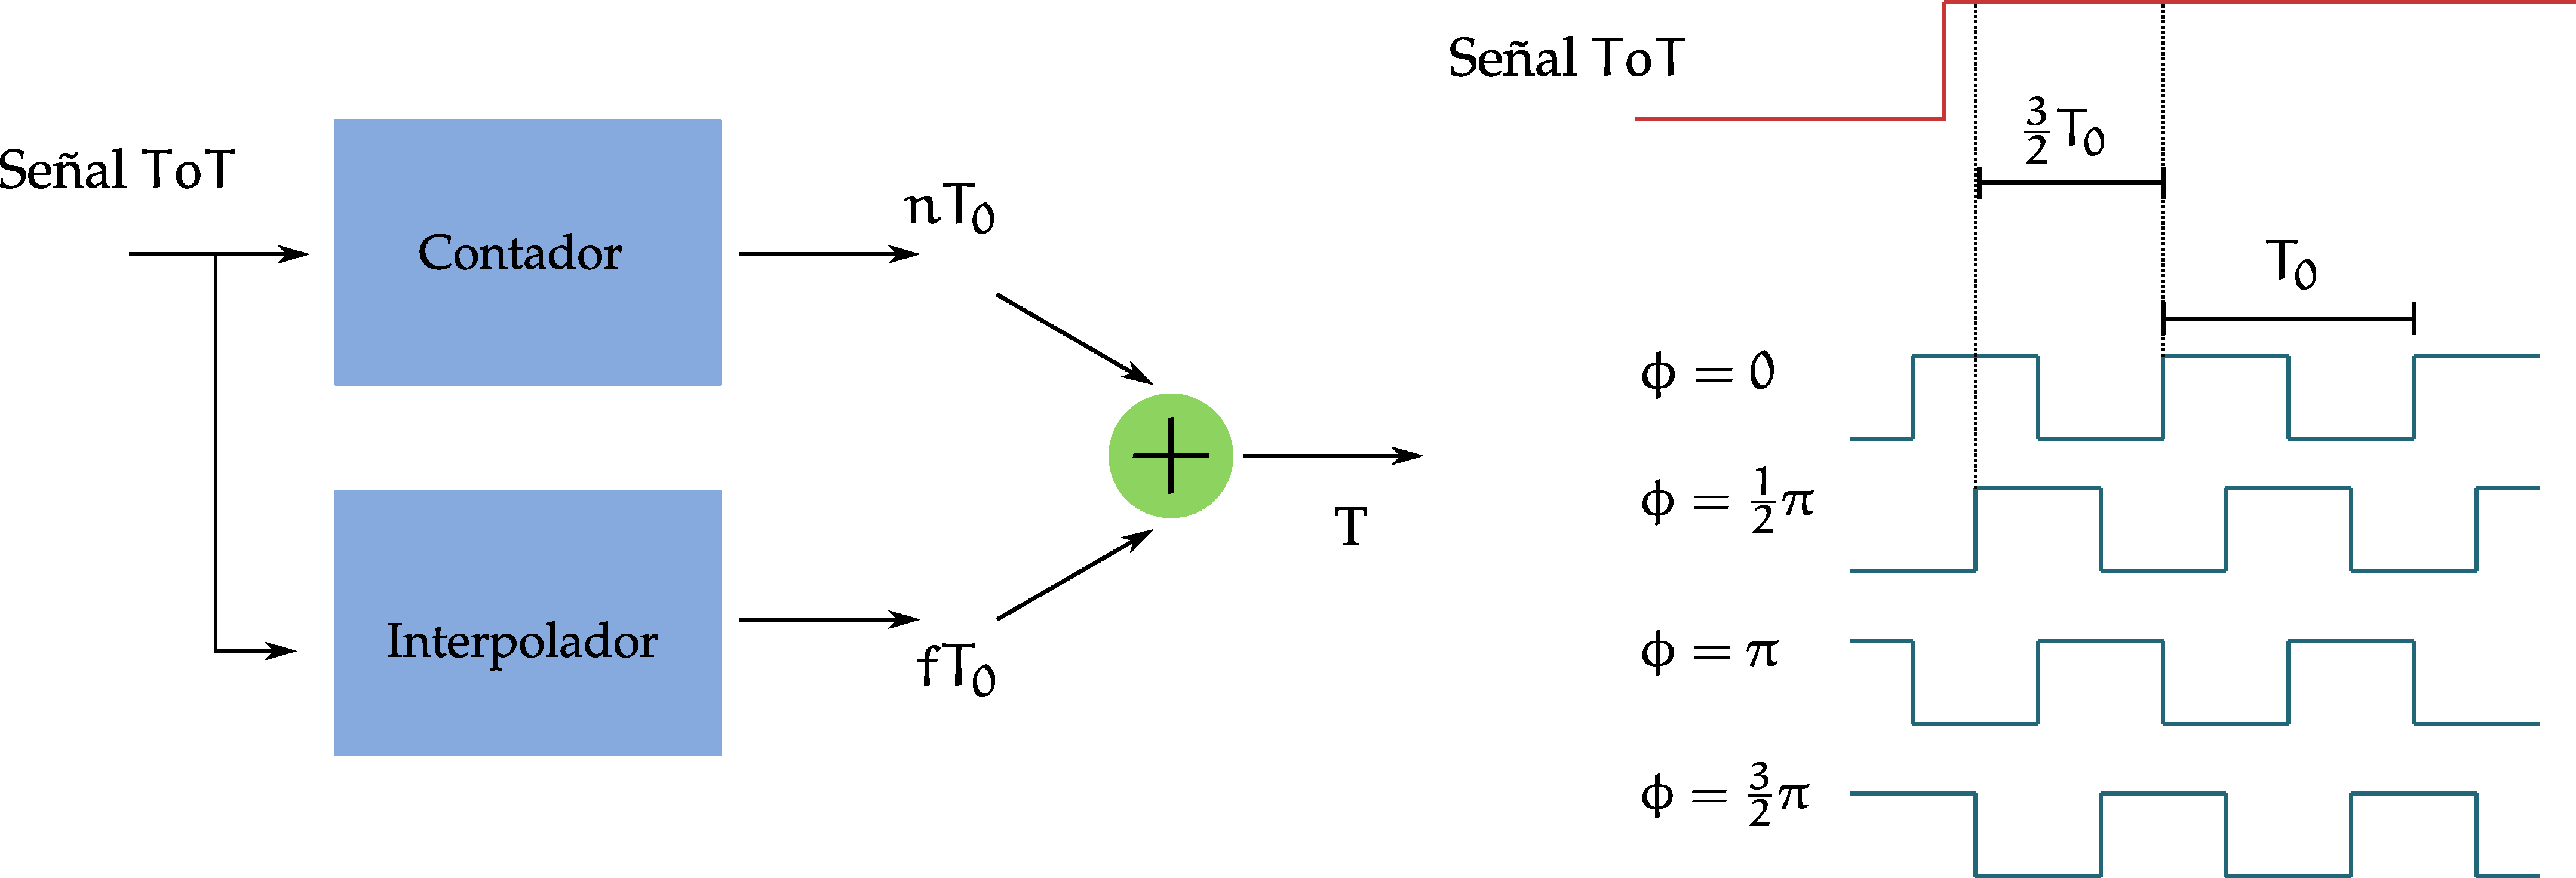
\includegraphics[width=\textwidth]{tdc-diagram.pdf}
        \caption{Arquitectura básica del sistema TDC por interpolación (panel izquierdo). Diagrama de tiempo y principio de operación del sistema TDC por interpolación.}
        \label{fig:tdc-diagram}
\end{figure}
